\documentclass{article}
\usepackage[utf8]{inputenc}
\usepackage{tikz}
\usepackage{verbatim}
\usepackage[bottom=2.0cm,top=2.0cm,left=1.7cm,right=1.7cm]{geometry}
\documentclass[tikz,margin=2mm]{standalone}
\usetikzlibrary{trees,arrows}

\title{TP2-IFT3913}
\author{Wenhao Xu, 20150702\\Manping Li, 968527}
\date{}


\begin{document}

\maketitle

\section*{Tâche 1}

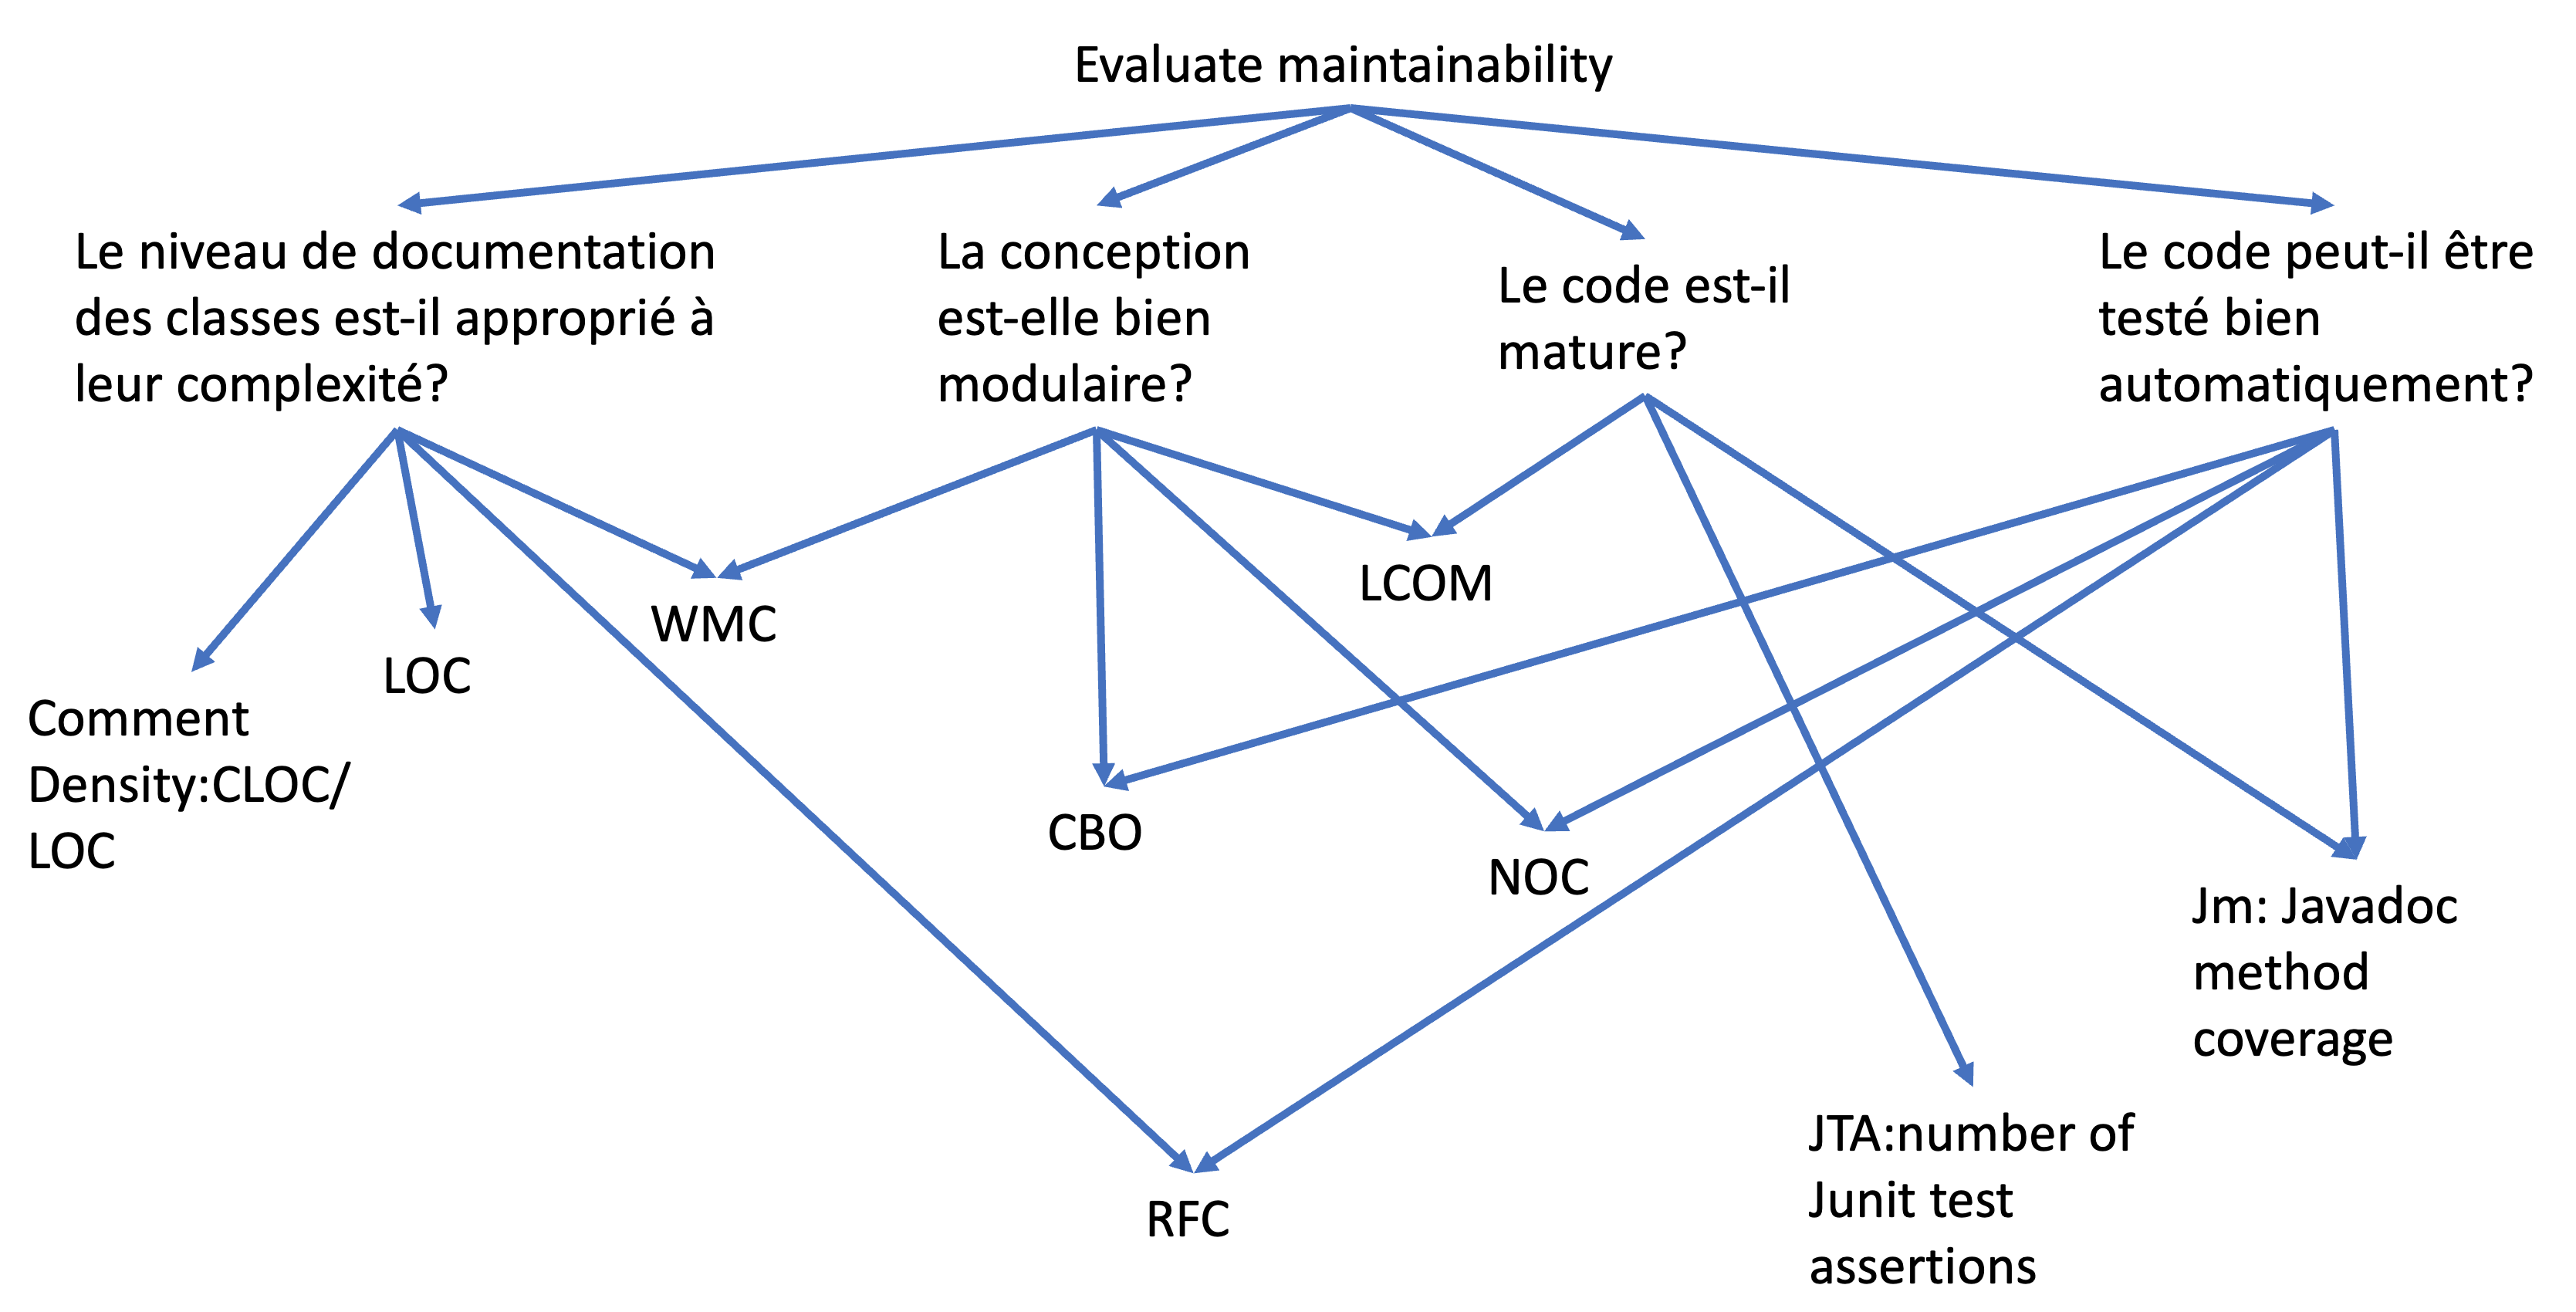
\includegraphics[width=0.95\textwidth]{GQM.png}\cite{ref 1 }\\\\
LOC\\
-Indique le nombre approximatif de lignes dans le code. Plus de lignes de code indiquent que la méthode spécifique peut effectuer beaucoup de tâches et peut violer le principe de responsabilité unique. Cela peut également indiquer que le logique de code n'est pas bien écrite ou n'est pas optimisée. Il faut donc essayer de le décomposer au maximum pour qu'il devienne plus réutilisable, plus propre et moins complexe.\\
Densité de commentaires\\
-La densité de commentaires est le pourcentage de lignes de commentaires dans une base de code source donnée, c'est-à-dire les lignes de commentaires divisées par le nombre total de lignes de code. La densité des commentaires est supposée être un bon prédicteur de la maintenabilité.Le plus la densité de commentaires est élevé le plus le code est biens documenté et donc plus facile à maintenir.c'est une metrics qui est à la fois mesure le niveau de documentation et le niveau de complexité.\\
WMC\\
- Le nombre de méthodes et la complexité des méthodes impliquées est un prédicteur du temps et des efforts nécessaires pour développer et maintenir la classe. Plus le nombre de méthodes dans une classe est grand, plus l'impact potentiel sur les enfants est important.Celi est un indicateur de mauvaise modularité. Les classes avec un grand nombre de méthodes sont susceptibles d'être plus spécifiques à l'application, ce qui limite la possibilité de réutilisation.\\
CBO\\
-Un couplage fort complique un système car une classe est plus difficile à comprendre, à modifier ou à corriger par elle-même si elle est interdépendante avec d'autres classes. La complexité peut être réduite en concevant des systèmes avec le couplage le plus faible possible entre les classes. Cela améliore la modularité et favorise l'encapsulation.l'effort de test d'une classe sera d'autant plus élevé que le CBO de cette classe est élevé.\\
LCOM\\
-Le manque de cohésion ou une faible cohésion augmente la complexité, augmentant ainsi la probabilité d'erreurs au cours du processus de développement.Ceci indique le logiciel n'est pas encore mature. \\
RFC\\
-Plus le nombre de méthodes pouvant être invoquées à partir d'une classe via des messages est grand, plus la complexité de la classe est grande. Si un grand nombre de méthodes peuvent être invoquées en réponse à un message, le test et le débogage de la classe deviennent compliqués car ils nécessitent un plus grand niveau de compréhension de la part du testeur. \\
Jm\\
- Une classe testable mature doit avoir une bonne couverture Javadoc pour s'assurer que ses méthodes de fonction peuvent être bien comprises et déboguées pour une modification et une maintenance ultérieures.\\
NOC\\
- Si une classe a un grand nombre d'enfants, cela peut nécessiter plus de tests des méthodes de cette classe, augmentant ainsi le temps de test.\\
JTA\\
- Un programme mature doit être simulé et testé avec presque 0 assertion (pas d'erreur).\\

\section*{Tâche 2}
Après avoir essayé plusieurs testeurs de métriques, nous avons finalement choisi le plugin MetricsReloaded d'IntelliJ comme programme de test. Non seulement il est très complet en termes de métriques qu'il teste, mais il est également facile à installer et à utiliser. Nous avons choisi LOC comme notre propre métrique à implémenter.Nous avons premièrement parser le code pour charque class et puis nous avons calculé la ligne de code total pour chaque class.\\


En raison de contraintes d'espace, les détails sur la façon de l'utiliser sont écrits dans le fichier readme.txt.

\section*{Tâche 3}
Nous avons implémenté un programme de jugement appelé MetricsCheck pour juger les 4 questions par rapport aux données exportées dans la partie2 (fichiers .csv). Nous avons pris une valeur moyenne pour chaque métrique (sauf pour Jm et JTA qui ont fixé un seuil fixe de 90\% de couverture et 0 assertion) et avons ensuite comparé chaque classe à cette valeur moyenne pour déterminer si elle était supérieure ou inférieure à cette valeur moyenne, générant ainsi la proportion de fichiers qui remplissaient la condition. Enfin, nous faisons la moyenne des proportions de plusieurs métriques correspondant à chaque enjeu pour déterminer si elles sont supérieures au pourcentage $<seuil>$, et si c'est le cas, nous considérons que cette condition d'enjeu est satisfaite.\\
Au début, nous avons utilisé 90\% comme $<seuil>$ pour l'évaluation, mais nous avons fini par obtenir un résultat où aucune des 4 questions n'était satisfaite, ce qui était un peu étrange, car $jfreechart$, étant un projet relativement mature, ne devrait pas avoir autant de questions. Nous avons pensé que le $<seuil>$ était peut-être un peu strict, alors nous sommes passés à 80\% et nous nous sommes retrouvés avec un "Oui" pour les Q3 et Q4.\\
Malgré les résultats obtenus, nous ne considérons pas qu'il s'agisse de l'évaluation finale de la maintenabilité. Les quatre questions sur la maintenabilité sont quelque peu vagues et nous n'avons pas été en mesure de trouver une métrique précise pour elles, seulement quelques unes relativement pertinentes, et certains des logiciels de test professionnel actuellement disponibles sur le marché sont incapables de fournir des réponses précises à ces questions. Les métriques que nous avons choisies sont relativement classiques, mais avec le développement continu de la théorie et de la technologie, des métriques plus complexes seront créées pour donner des réponses plus précises. Dans l'ensemble, les tests de logiciels sont un processus d'amélioration et de développement continu, et nous devons évaluer certains paramètres de manière dynamique.
\begin{thebibliography}{}  
 
     \bibitem{ref 1 }\\
        Powered by MetricsReloaded\\
        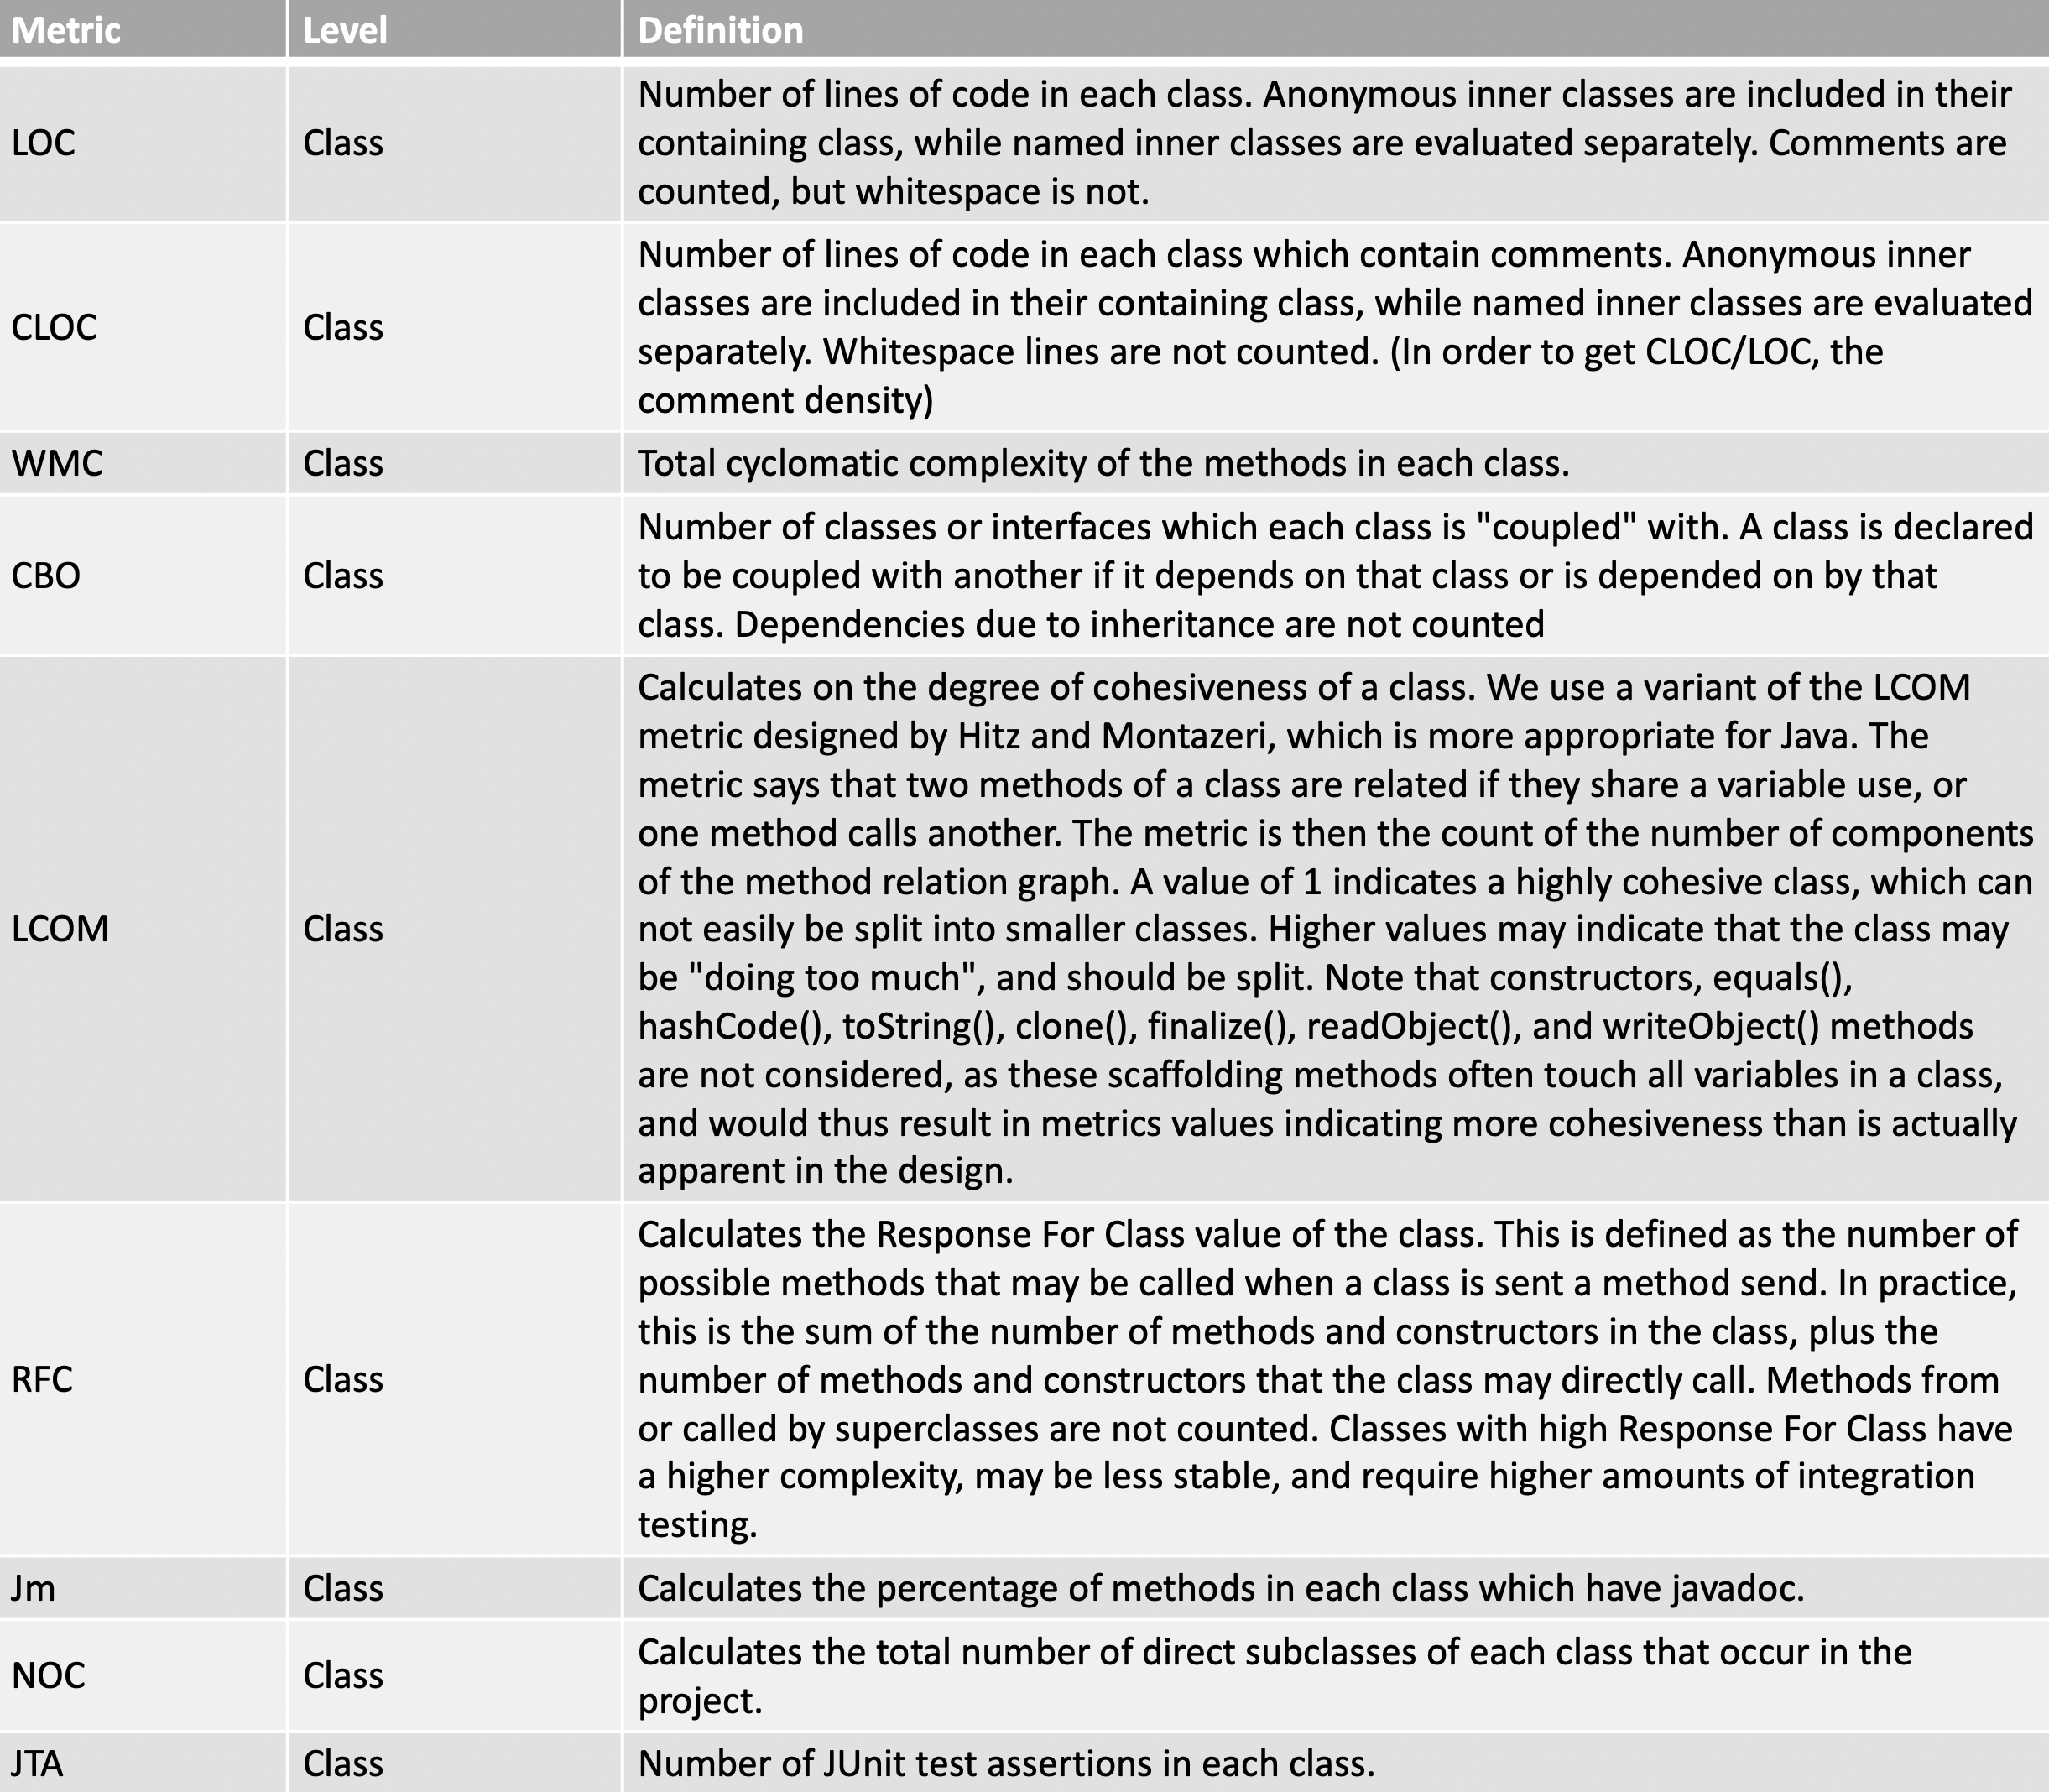
\includegraphics[width=0.95\textwidth]{Defi.png}
        
 
\end{thebibliography}


\end{document}
